\block{Motivations}{
		\begin{minipage}{0.48\linewidth}
			\textbf{Current Objective :} Develop hybrid \textbf{\fcolorbox{color1!50}{color1}{finite element}} / \textbf{\fcolorbox{color1!50}{color1}{neural network}} methods.
		
			\vspace{-5pt}
			\hspace{480pt} \begin{minipage}{0.5\linewidth}
				\textbf{\textcolor{color2}{accurate}}
				\hspace{25pt}
				\textbf{\textcolor{color2}{quick + parameterized}}
			\end{minipage}
			
		\end{minipage}
		\begin{minipage}{0.46\linewidth}
			\centering
			\textbf{Problem considered :} $\qquad -\Delta u(X,\mu) = f(X,\mu) \quad \text{in } \Omega\times\mathcal{M}, \quad u(x,\mu) = 0 \quad \text{on } \Gamma\times\mathcal{M}.$ \\
			Poisson problem with homogeneous Dirichlet boundary conditions (BC).
		\end{minipage}
		
		\vspace{20pt}
		
		\begin{center}
			\begin{minipage}{0.395\linewidth}
				\centering
				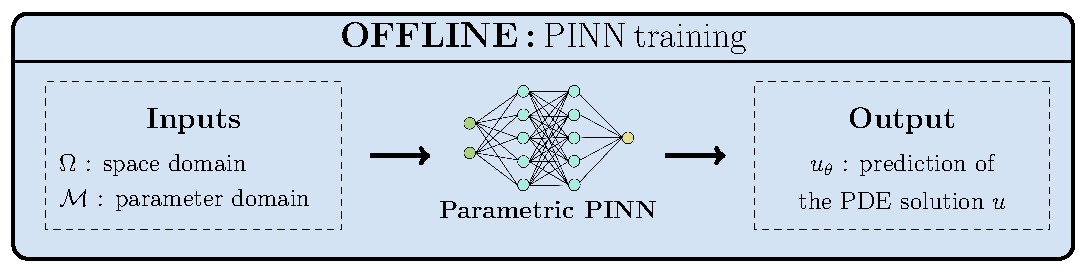
\includegraphics[width=\linewidth]{images/intro/offline.pdf}
			\end{minipage}	
			\begin{minipage}{0.595\linewidth}
				\centering
				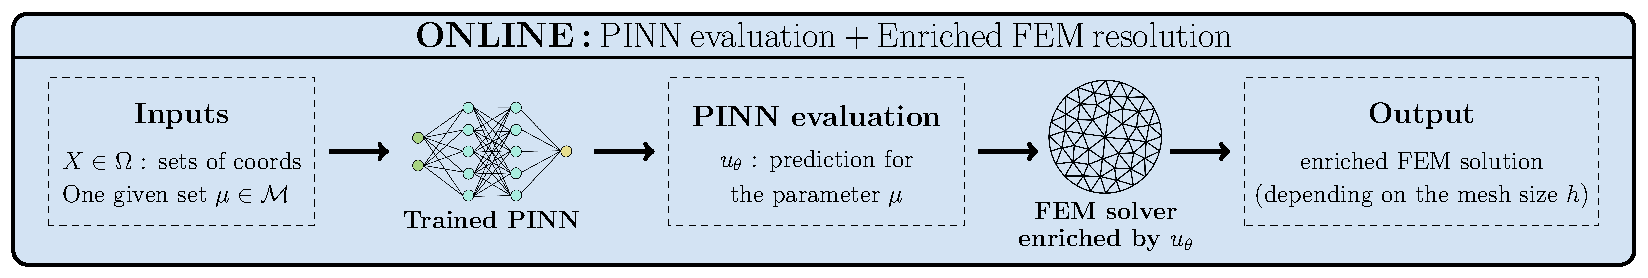
\includegraphics[width=\linewidth]{images/intro/online.pdf}
			\end{minipage}
		\end{center}		
	
		\vspace{20pt}

		\textbf{Perspective :} Create real-time digital twins of an organ (e.g. liver).
		\vspace{-20pt}
}
		
\node[rotate=-30,below left=0.5cm and -0.5cm] at (topright) {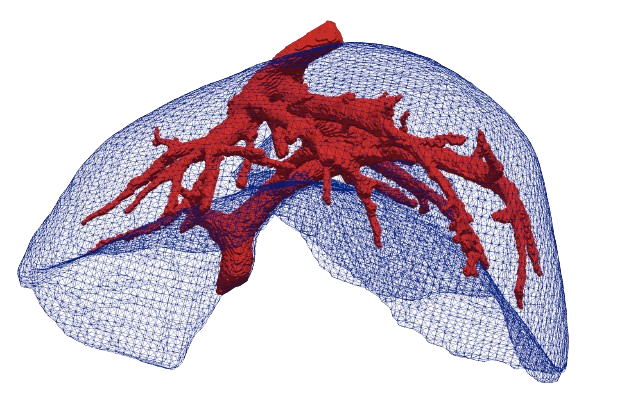
\includegraphics[width=9cm]{images/intro/foie.png}};